\section{Copolimeri a blocchi accettore-donatore}% - punto di vista accettore}
\nsub{I polimeri elettron-accettori}\footnotetext{\tiny{\cite{5}DOI: 10.1021/ma102566u}}
Il materiale elettron-accettore (di tipo~n) più usato è fullerene funzionalizzato PCBM (è solubile ed ha ottime proprietà di elettron-accettore e trasportatore di elettroni) oppure nanoparticelle inorganiche.

A causa della sua simmetria il fullerene ha assorbimento solo ad alte energie.

L'alternativa di impiegare polimeri coniugati elettron-accettori porta a grossi problemi di smescolamento.
\begin{columns}\column{0.5\linewidth}
\begin{figure}{\centering{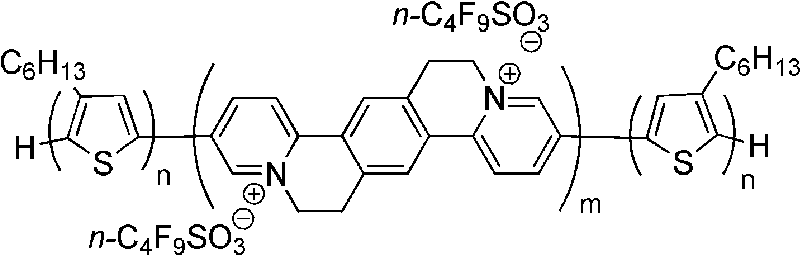
\includegraphics[width=1\textwidth]{img/dba-piridin-tio.png}}}\end{figure}\column{0.5\linewidth}
Esempio di polimero a blocchi donatore-accettore-donatore.

\end{columns}
\end{frame}



% %%%%%%%%%%%%%%%%%%%%%%%%%%%%%%%%%%%%%%%%%%%%%%%%%%%%%%%%%%%%%%%%%%%%%%%%%%%%%%%%%%%%%%%%%%%%%%%%%%%%%%%%%%%%%%%%%%%%%%%%%%%%%%

\nsub{Basati su fullerene}
Per evitare lo smescolamento del fullerene si può:
\begin{enumerate}
 \item fullerene legato alle catene laterali del polimero donatore (polimeri ``doppio cavo'') ma si ha ricombinazione di cariche;
 \item copolimero a blocchi donatore-(blocco con fullereni in catena laterale o al termine) non troppo funzionalizzato per garantire la percolazione ed evitare la reticolazione;
 \item copolimero a blocchi donatore-(polimero con gruppi leganti di fullereni);
 \item un copolimero a blocchi come compatibilizzante.
\end{enumerate}
Se la catena con i fullereni è non coniugata fungerà da isolante. Al contrario se è coniugata si ha un migliore trasferimento\\(\emph{quenching} di fotoluminescenza).
 \end{frame}

\subsubsection{Esempi di accettori con fullereni}\begin{frame}\frametitle{Basati su fullerene}\framesubtitle{Esempi di accettori con fullereni}
\begin{figure}{\centering{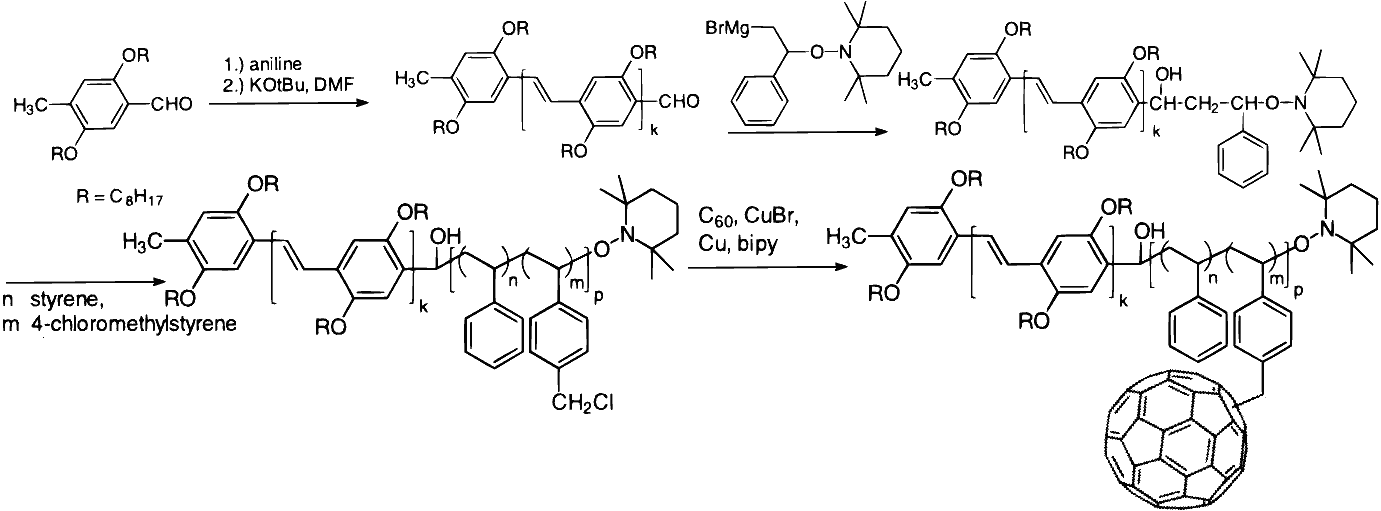
\includegraphics[width=0.8\textwidth]{img/dba-fu-ps-ppv.png}}}\end{figure}\vspace{-30pt}{\tiny{\cite{2}DOI: 10.1021/ja000160a}} 
\begin{figure}{{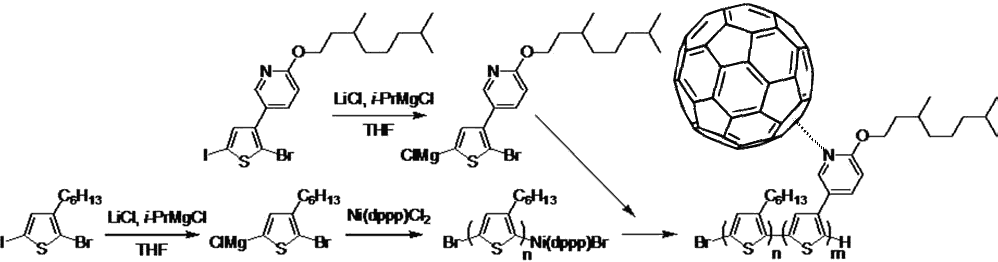
\includegraphics[width=0.8\textwidth]{img/dba-fu-tio-tioleg.png}}}\end{figure}\tiny{\cite{3}DOI: 10.1002/pola.24689} 
\end{frame}


\subsubsection{Polimeri a blocchi come compatibilizzanti}\begin{frame}\frametitle{Basati su fullerene}\framesubtitle{Polimeri a blocchi come compatibilizzanti}
\footnotetext{\tiny{\cite{6}DOI: 10.1002/macp.201000080}}
\begin{columns} \column{0.5\linewidth}
I polimeri a blocchi possono essere utilizzati come compatibilizzanti di miscele polimero-fullerene o polimero donatore-polimero accettore. 
\column{0.5\linewidth}\vspace{-10pt}\begin{figure}{\centering{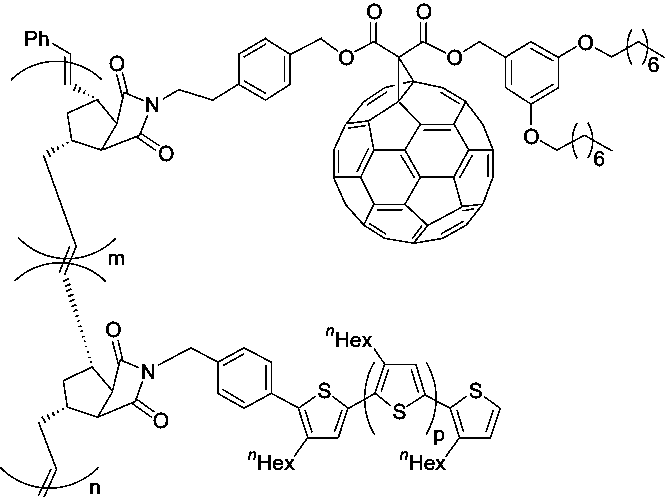
\includegraphics[width=0.9\textwidth]{img/dba-fu-tio.png}}}
\end{figure}\tiny{\cite{9}DOI: 10.1002/adma.200501787}
\end{columns}
\begin{figure}{{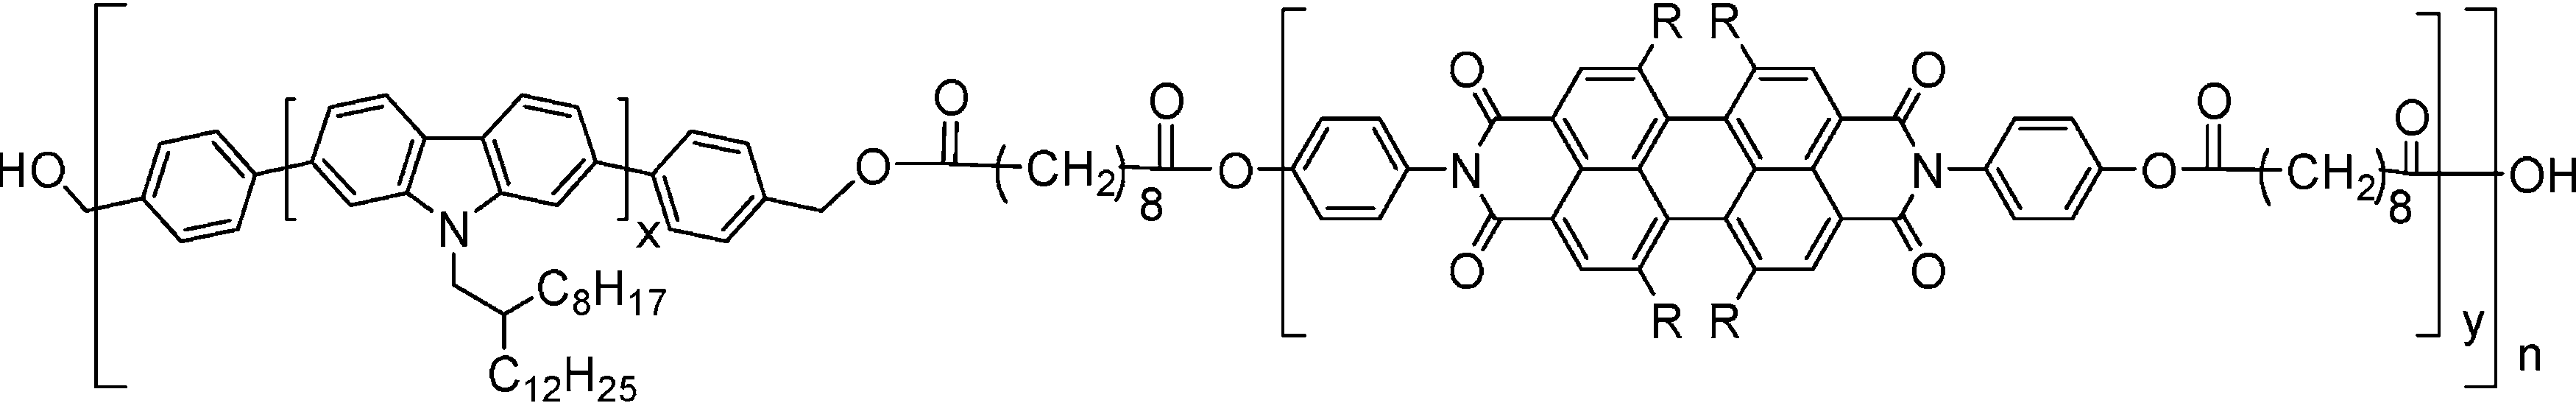
\includegraphics[width=0.9\textwidth]{img/dba-spacer.png}}}\end{figure}
\end{frame}

% %%%%%%%%%%%%%%%%%%%%%%%%%%%%%%%%%%%%%%%%%%%%%%%%%%%%%%%%%%%%%%%%%%%%%%%%%%%%%%%%%%%%%%%%%%%%%%%%%%%%%%%%%%%%%%%%%%%%%%%%%%%%%%
\nsub{Basati su perilene bisimmide}
\small{La eccessiva cristallizzazione del perilene bisimmide può essere limitata impiegandolo in un polimero a blocchi. La sintesi NMRP in figura usa come donatore tetrafenilbenzidina (HOMO e LUMO adatti, mobilità di lacune maggiore della trifenilammina (ma peggior macroiniziatore), i sostituenti donatori metossi aumentano la solubilità ed innalzano il HOMO).}
\begin{figure}{\centering{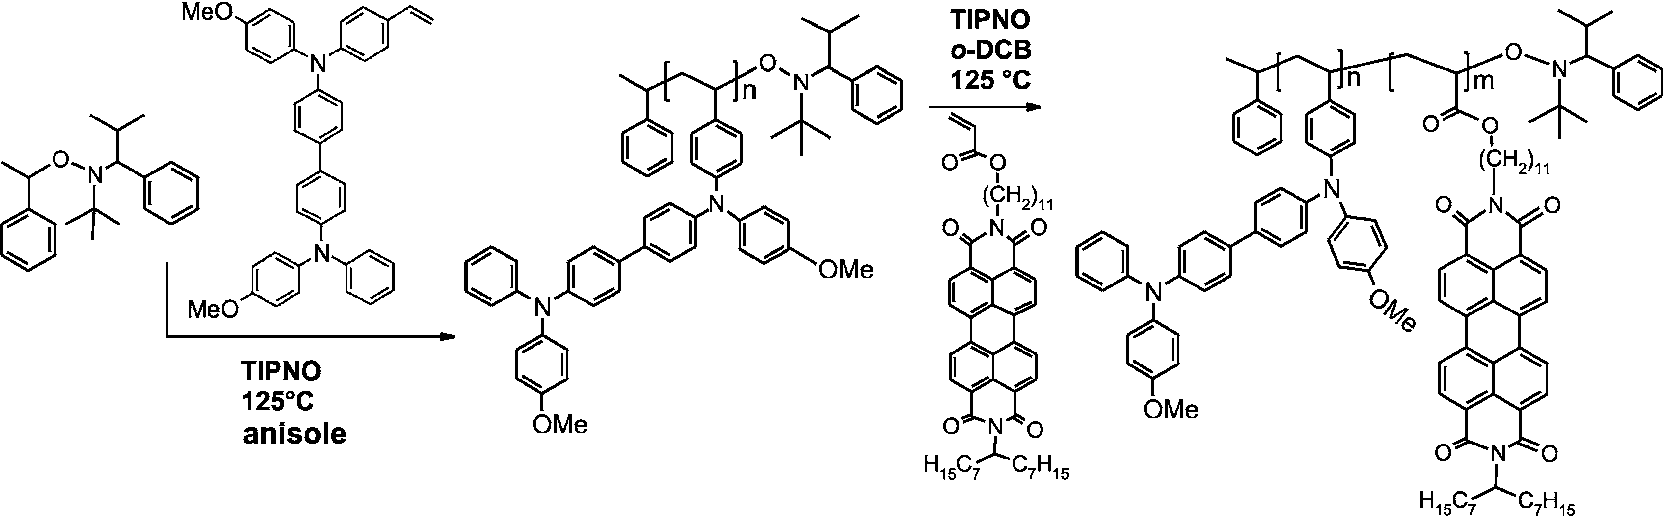
\includegraphics[width=1\textwidth]{img/dba-pbi-vtpa.png}}}
\end{figure}\vspace{-10pt}{\tiny{\cite{10}DOI: 10.1007/12\_2009\_34}}
\end{frame}

% %%%%%%%%%%%%%%%%%%%%%%%%%%%%%%%%%%%%%%%%%%%%%%%%%%%%%%%%%%%%%%%%%%%%%%%%%%%%%%%%%%%%%%%%%%%%%%%%%%%%%%%%%%%%%%%%%%%%%%%%%%%%%%

\nsub{Basati su $p$-fenilene vinilene}
Il carattere elettron-attrattore può essere proprio del monomero (come nel PBI o nel fullerene) oppure derivare da comonomeri o da modifiche strutturali su polimeri conduttori già visti.
\begin{figure}{{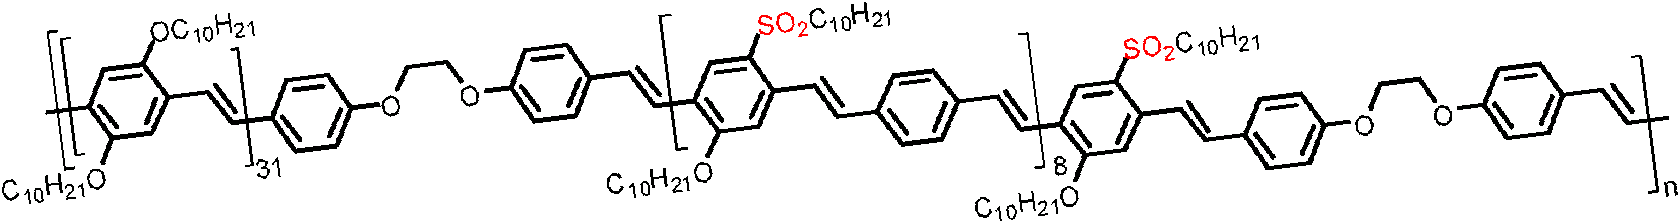
\includegraphics[width=0.9\textwidth]{img/dba-ppv-so2.png}}}\end{figure}\vspace{-10pt}{\tiny{\cite{7}DOI: 10.1063/1.2437100}}\\
CN abbassa HOMO e LUMO. In assenza di catene laterali sul blocco accettore Y è molto basso.
\begin{figure}{{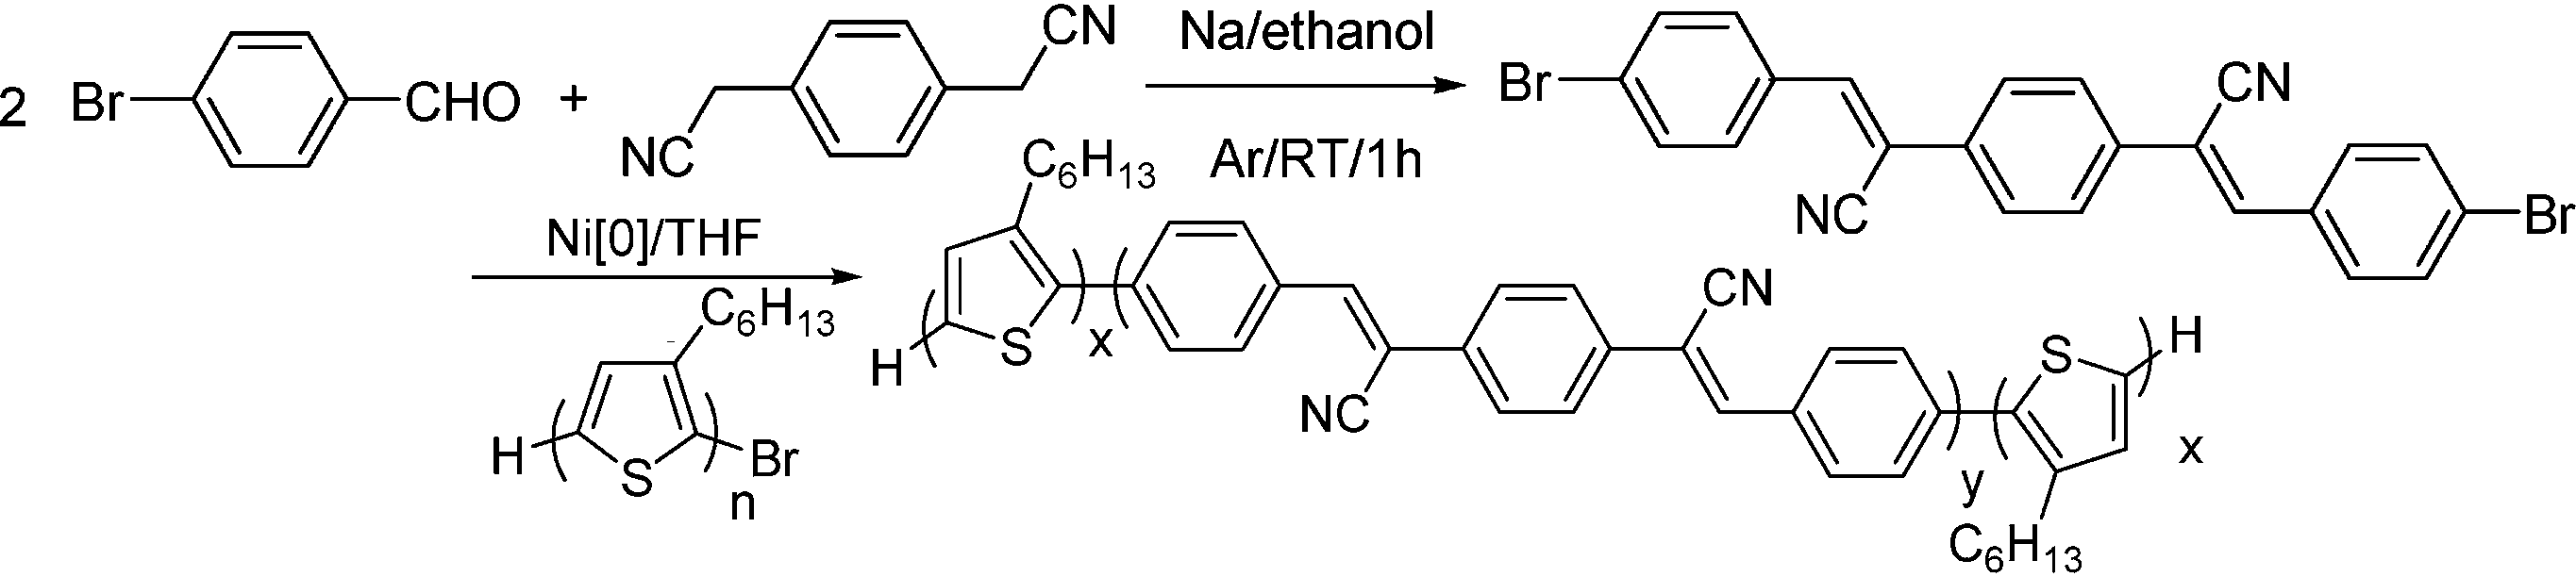
\includegraphics[width=0.8\textwidth]{img/dba-ppv-cn-tio.png}}}\end{figure}\vspace{-10pt}\tiny{\cite{8}DOI: 10.1021/ma060341i}

\end{frame}
% %%%%%%%%%%%%%%%%%%%%%%%%%%%%%%%%%%%%%%%%%%%%%%%%%%%%%%%%%%%%%%%%%%%%%%%%%%%%%%%%%%%%%%%%%%%%%%%%%%%%%%%%%%%%%%%%%%%%%%%%%%%%%%

\nsub{Basati su fluorene}In politiofene-$b$-polifluorene il polifluorene può essere utilizzato come elettron-accettore.
\begin{columns} \column{0.7\linewidth} Per facilitare l'auto-organizzazione si può rendere polare un blocco. In solventi di diversa polarità si avranno micelle o micelle inverse.
\column{0.25\linewidth}
\begin{figure}{{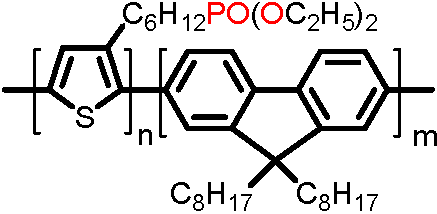
\includegraphics[width=1\textwidth]{img/dba-fluo-tiop.png}}}\\\vspace{-5pt}{\tiny{\cite{1}DOI: 10.1021/ar7002539}}\end{figure}
\column{0.05\linewidth}\end{columns}\vspace{10pt}
Copolimerizzando fluorene con benzotiadiazolo in modo \emph{random} utilizzando Suzuki si ottiene un miglior elettron-accettore. 
\begin{figure}{{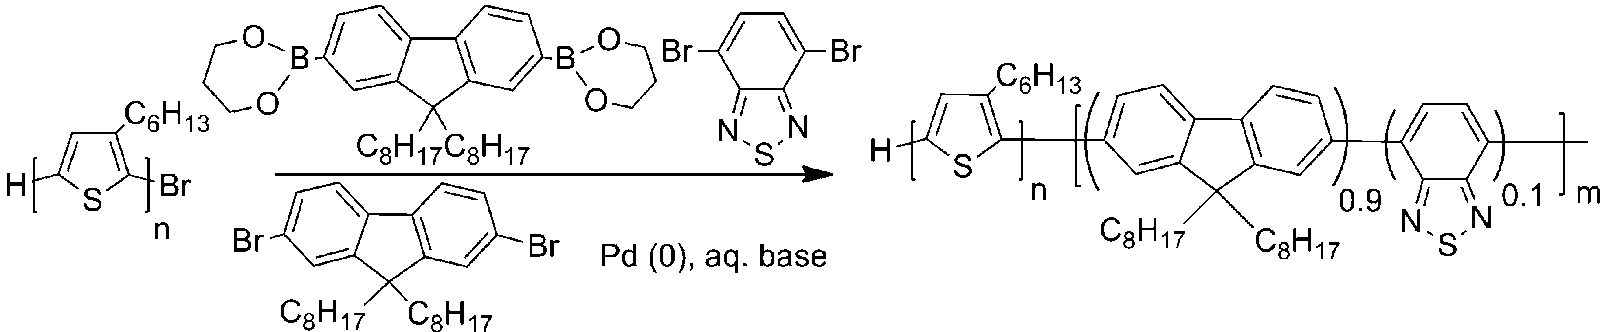
\includegraphics[width=0.8\textwidth]{img/dba-fluo-tio.png}}}\end{figure}\vspace{-5pt}{\tiny{\cite{4}DOI: 10.1021/ma102728z}}

\end{frame}
